% amd_india_opperunites.tex
% GTAC 2026 double-blind submission
% Title: Voice-AI: AMD, India Business Opportunities: A Techno-Business Study

\documentclass[blind]{gtac}

\usepackage{cite}
\usepackage{xcolor}
\usepackage{booktabs}
\usepackage{float}
\usepackage{tikz}
\usetikzlibrary{arrows.meta,positioning}
\usepackage[colorlinks=true, linkcolor=blue, urlcolor=blue, citecolor=blue]{hyperref}
\Urlmuskip=0mu plus 1mu\relax % allow long URLs in references to break
\providecommand{\rupee}{\ensuremath{\text{\rm\textsf{R}}}} % lightweight rupee marker
\renewcommand{\rupee}{Rs.\,} % use "Rs." to avoid font dependencies

\SetWatermarkScale{0.3}
\SetWatermarkAngle{30}
\SetWatermarkColor{gray!20}

\title{{Voice-AI: AMD, India, and the Business Opportunity --- A Techno-Business Study}}

\author{Anonymous}

\begin{document}

\maketitle

\pagestyle{fancy}
\fancyhf{}
\cfoot{\thepage}
\renewcommand{\headrulewidth}{0pt}
\chead{{\sffamily\textcolor{red}{\fontsize{10}{12}\selectfont\textbf{DO NOT FORWARD -- FOR GTAC'26 REVIEW COMMITTEE ONLY}}}}
\thispagestyle{fancy}

\begin{abstract}
Voice AI has moved from research curiosity to production infrastructure: the AI voice-agents market is projected to grow from \$2.4B in 2024 to \$47.5B by 2034 at a 35\% CAGR, venture funding reached \$2.1B in 2025 (8$\times$ the 2022 level), and production deployments grew 340\% year-over-year across 500+ organizations~\cite{grandview,assemblyai_2026}. A deployed voice agent is a \emph{steady-state inference machine} that transcribes, reasons, and speaks 24/7 at roughly \$0.40 per call versus \$7--\$12 for a human agent---and at scale its dominant operating cost is GPU compute. This paper presents a techno-business assessment of where AMD can win in this market, with a particular focus on India as a strategic beachhead and a template for global scale. We show that AMD holds a demonstrable inference cost advantage---34\% lower cost-per-token for 70B-class LLMs on MI300X versus H100, single-GPU fit for models that otherwise need two H100s, and $\sim$50\% lower list price for equivalent capability---yet captures little of the market because the value chain selects hardware \emph{implicitly} through frameworks, containers, domain SDKs, edge modules, cloud marketplace slots, and systems-integrator channels where NVIDIA is already positioned. We analyze eight verticals (BFSI, healthcare, contact centers, manufacturing, automotive, retail, education, government) for market size, ease of entry, required partnerships, and adoption horizon; make the case for India---22 official languages, the second-largest concentration of voice-AI startups, and a data-residency regime (DPDP) that mandates on-premise deployment---as the natural entry point; extend the analysis to voice-plus-vision robotics and one-device edge intelligence; and close with a prioritized short/medium/long-term roadmap. The central thesis: AMD's opportunity is not a silicon problem but a \emph{go-to-market and ecosystem} problem, and the on-premise, compliance-constrained, cost-sensitive segments---anchored in India---are where AMD's structural advantages convert to revenue first.
\end{abstract}

\keywords{Voice AI, AMD, India, MI300X, ROCm, Ryzen AI, market strategy, BFSI, DPDP, edge AI, robotics, techno-business analysis.}

%---------------------------------------------------------------------------
\section{Introduction}
\label{sec:intro}
%---------------------------------------------------------------------------

Voice AI agents now answer phones, qualify leads, triage patients, schedule appointments, and run collections. Unlike a trained model that is an artifact, a deployed voice agent is an always-on service: it does not train, it \emph{serves}, continuously converting speech to text, text to intent, intent to reply, and reply to speech. The economics are compelling---a voice AI call costs approximately \$0.40 against \$7--\$12 for a human agent, a 90--95\% reduction~\cite{assemblyai_2026,grandview}---and the market has responded. Gartner projects voice AI will cut contact-center labor costs by \$80B in 2026 alone, and 80\% of customer-service organizations plan a voice deployment by the end of that year~\cite{assemblyai_2026}.

At scale, the dominant recurring cost of a voice agent is GPU compute in three layers---automatic speech recognition (ASR), the large language model (LLM), and text-to-speech (TTS). This is precisely where hardware economics decide platform margins, and precisely where AMD holds a measurable advantage: the MI300X delivers 34\% lower cost-per-token than the NVIDIA H100 and fits a 70B-class model on a single 192\,GB device that would otherwise require two H100s~\cite{spheron_rocm,vllm_rocm}. Yet AMD is largely absent from voice AI production, not because its silicon underperforms, but because the market selects compute \emph{before} anyone consciously chooses a GPU---through orchestration frameworks, pre-packaged inference containers, voice-domain SDKs, embedded edge modules, cloud marketplace dropdowns, and the delivery playbooks of systems integrators.

This paper is a techno-business study of that opportunity. We ask four questions: (1) How large is the market and how fast is it growing, globally and in India? (2) Where, specifically, can AMD compete, and which segments are easy versus hard to enter? (3) Why is India uniquely positioned as a beachhead that scales to the world? (4) What is the concrete action roadmap---which customers, which collaboration layers, which timelines? Sections~\ref{sec:landscape}--\ref{sec:amd} establish the market and AMD's position; Section~\ref{sec:india} makes the India case; Section~\ref{sec:sectors} analyzes eight verticals; Sections~\ref{sec:ecosystem}--\ref{sec:robotics} cover ecosystem strategy, one-device hardware, and robotics; Section~\ref{sec:competitive} is the competitive analysis; and Sections~\ref{sec:reco}--\ref{sec:conclusion} give recommendations and conclusions.

%---------------------------------------------------------------------------
\section{The Voice AI Market Landscape}
\label{sec:landscape}
%---------------------------------------------------------------------------

\subsection{Market Size and Growth}

Two market definitions matter. The broader voice-recognition market was \$18.39B in 2025 and is projected to reach \$61.71B by 2031 (22\% CAGR). The narrower, faster AI voice-agents market---the autonomous conversational systems this paper concerns---was \$2.4B in 2024 and is projected at \$47.5B by 2034 (35\% CAGR)~\cite{grandview}. Capital has followed: venture funding hit \$2.1B in 2025, 8$\times$ the 2022 level, and 2026 is already tracking 68\% above the 2025 pace~\cite{assemblyai_2026}. Consumer surface area is enormous---4.2B active digital voice assistants in 2024, projected to exceed 8.4B by 2028.

\begin{table}[H]
\centering
\caption{Voice AI market by region (2025 revenue share and growth).}
\label{tab:region}
\tiny
\begin{tabular}{@{}lcc@{}}
\toprule
Region & Revenue share & CAGR \\
\midrule
North America & 40--42\% & $\sim$28\% \\
Asia-Pacific & 28--34\% & \textbf{33--41\%} (fastest) \\
Europe & 19\% & $\sim$20\% \\
Middle East \& Africa & 5\% & 17--22\% \\
Latin America & emerging & $\sim$25\% \\
\bottomrule
\end{tabular}
\end{table}

North America leads on revenue (40.6\% of global), but Asia-Pacific is the fastest-growing region, with the voice-agents segment there projected at a 41.2\% CAGR through 2034---the single fastest global sub-segment. The geographic distribution of \emph{builders} mirrors this: the US hosts 62 voice AI startups, India 32 (second globally), and the UK 11~\cite{assemblyai_2026}.

\subsection{An Adoption Gap That Signals Headroom}

A telling asymmetry: 55\% of consumers now use voice to interact with AI, but only 29\% of companies have deployed customer-facing voice AI. Demand precedes supply. Analyst expectations underline the runway: Gartner forecasts that agentic AI will autonomously resolve 80\% of common customer-service issues by 2029 (cutting operational costs 30\%), and that 40\% of enterprise applications will integrate task-specific AI agents by end-2026, up from under 5\% in 2025~\cite{assemblyai_2026}. The market is early, the direction is set, and the hardware substrate for it is not yet locked.

\subsection{The Tech Stack: Where the Cost Lives}

A voice conversation traverses five layers (Figure~\ref{fig:pipe}). Telephony/transport and orchestration are I/O- and control-bound and carry little GPU cost. ASR, LLM, and TTS consume GPU cycles every conversation---this is the compute-bearing core and the locus of both AMD's advantage and its gap. The 2026 production latency median is 680\,ms (down from 1{,}200\,ms in 2024); the emerging bar is sub-500\,ms, which is especially tight on Indian cellular networks that add $\sim$50\,ms over fiber and degrade audio to 8\,kHz~\cite{assemblyai_stack}.

\begin{figure}[H]
\centering
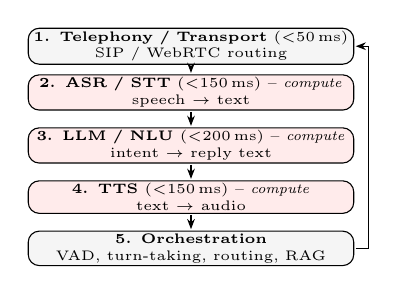
\begin{tikzpicture}[
  font=\tiny,
  box/.style={draw, rounded corners, align=center, text width=1.6in,
              minimum height=2.6ex, inner sep=1pt},
  comp/.style={box, fill=red!8},
  light/.style={box, fill=gray!8},
  arr/.style={-{Stealth[length=1.3mm]}, shorten >=0.5pt, shorten <=0.5pt}
]
\node[light] (tel) {\textbf{1. Telephony / Transport} ($<$50\,ms)\\ SIP / WebRTC routing};
\node[comp, below=0.8ex of tel] (asr)
  {\textbf{2. ASR / STT} ($<$150\,ms) -- \emph{compute}\\ speech $\rightarrow$ text};
\node[comp, below=1.4ex of asr] (llm)
  {\textbf{3. LLM / NLU} ($<$200\,ms) -- \emph{compute}\\ intent $\rightarrow$ reply text};
\node[comp, below=1.4ex of llm] (tts)
  {\textbf{4. TTS} ($<$150\,ms) -- \emph{compute}\\ text $\rightarrow$ audio};
\node[light, below=1.4ex of tts] (orc)
  {\textbf{5. Orchestration}\\ VAD, turn-taking, routing, RAG};
\draw[arr] (tel) -- (asr);
\draw[arr] (asr) -- (llm);
\draw[arr] (llm) -- (tts);
\draw[arr] (tts) -- (orc);
\draw[arr] (orc.east) -- ++(0.18,0) |- (tel.east);
\end{tikzpicture}
\caption{The five-layer voice pipeline with per-layer latency budget. Shaded layers
(ASR, LLM, TTS) are GPU-compute-bearing---where hardware economics and AMD's
opportunity both reside.}
\label{fig:pipe}
\end{figure}

Table~\ref{tab:stackcost} shows the monthly cost per 10{,}000 minutes. Two facts drive the business case. First, LLM inference is the cheapest layer per minute but the most latency-critical (first token in $<$200\,ms). Second, TTS is the \emph{hidden budget killer}: premium hosted synthesis runs \$0.10--\$0.30/min and can exceed ASR and LLM combined, which is why self-hosted GPU-resident TTS is economically decisive at scale~\cite{bentoml_tts,raftlabs_cost}. Both the LLM and TTS layers are where self-hosting on cost-efficient GPUs---AMD's advantage---matters most.

\begin{table}[H]
\centering
\caption{Full-stack cost per 10{,}000 minutes/month~\cite{raftlabs_cost,bentoml_tts}.}
\label{tab:stackcost}
\tiny
\begin{tabular}{@{}lcc@{}}
\toprule
Layer & DIY / self-hosted & Managed cloud \\
\midrule
Telephony & \$35--140 & \$35--140 \\
ASR / STT & \$15--50 (GPU) & \$43--240 \\
LLM & \$20--150 & \$20--150 \\
TTS & \$20--50 (GPU) & \textbf{\$200--3{,}000} \\
Infrastructure (GPU/cloud) & \$200--800 & included \\
\midrule
\textbf{Total} & \textbf{\$290--1{,}190} & \textbf{\$298--3{,}530} \\
\bottomrule
\end{tabular}
\end{table}

\subsection{Convergence: Three Frameworks Orchestrate Everything}

Despite hundreds of companies and billions in funding, production code has converged on three open-source orchestration frameworks; commercial platforms (Vapi, Retell, Bolna, PolyAI, Gnani, Sarvam, Caller Digital, Synthflow) are business layers above one of them:

\begin{itemize}
  \item \textbf{LiveKit Agents} (Apache 2.0)---WebRTC backbone used by OpenAI ChatGPT Voice Mode, Character.ai, and Meta; native SIP shipped 2025.
  \item \textbf{Pipecat} (BSD-2, Daily.ai, v1.0 April 2026)---Python frame-pipeline with 60+ swappable ASR/LLM/TTS/transport connectors.
  \item \textbf{TEN} (C++/Go/Python)---highest-performance option with proprietary VAD and sub-300\,ms turn-detection, avatar integration.
\end{itemize}

This convergence is strategically important: whoever wins the framework plugin slot and the container layer wins the hardware default for every platform above. That is the lever this paper argues AMD must pull.

%---------------------------------------------------------------------------
\section{AMD's Strategic Opportunity}
\label{sec:amd}
%---------------------------------------------------------------------------

\subsection{The Structural Hardware Advantage}

AMD's case rests on inference economics at the two heaviest compute layers. Table~\ref{tab:llm} shows the MI300X matching H100 throughput at materially lower cost, with a structural VRAM advantage: a 70B-class model needs two H100s (160\,GB combined) but fits on a single MI300X (192\,GB), halving node count and removing NVLink/interconnect complexity. The MI355X (288\,GB HBM3e) pushes further, landing within single-digit percentage points of NVIDIA's B200 on MLPerf Inference v6.0 server workloads~\cite{mlperf6}.

\begin{table}[H]
\centering
\caption{LLM inference: MI300X vs.\ H100 SXM5 (2026 figures)~\cite{spheron_rocm,vllm_rocm}.}
\label{tab:llm}
\tiny
\begin{tabular}{@{}lcc@{}}
\toprule
Dimension & MI300X & H100 SXM5 \\
\midrule
VRAM & \textbf{192\,GB} HBM3 & 80\,GB HBM3e \\
On-demand cloud price & \$1.50--2.50/hr & \$2.90/hr \\
Throughput (Llama 3.1 70B) & $\sim$18{,}000 tok/s & $\sim$19{,}500 tok/s \\
Cost / 1M tokens & \textbf{\$0.027} & \$0.041 \\
70B fits on 1 GPU? & \textbf{Yes} & No (needs 2) \\
\bottomrule
\end{tabular}
\end{table}

These advantages compound at voice-platform scale. A deployment handling 1M minutes/month generates roughly 6B LLM tokens/month; the MI300X saves approximately \$84K/month---\$50K--\$100K/year---versus H100 on LLM inference alone, and self-hosted ROCm TTS eliminates a further \$100K--\$300K/month in premium hosted synthesis. At 10M minutes/month the combined LLM+TTS advantage is worth roughly \$600K/year~\cite{spheron_rocm,vllm_rocm,bentoml_tts}. For on-premise deployments---mandatory in regulated Indian markets---AMD's $\sim$50\% lower GPU list price for equivalent capability is a direct CapEx advantage.

\subsection{Software Readiness: The CUDA Gap Is Largely Closed}

Critically, the porting burden that once blocked AMD adoption has mostly dissolved for voice workloads (Table~\ref{tab:compat}). LLM serving (vLLM, SGLang) and the leading self-hostable TTS models (Kokoro, Chatterbox) run on ROCm at 90--95\% of CUDA performance with little or no code change, because HIP transparently maps CUDA calls and these models are pure PyTorch~\cite{vllm_rocm,bentoml_tts}. vLLM ROCm became officially first-class in January 2026, with CI pass rate jumping from 37\% to 93\% in six weeks and a pre-built Docker image shipping. The remaining gaps---streaming ASR containers and HuggingFace Text-Embeddings-Inference (TEI) for RAG---are narrow and closeable.

\begin{table}[H]
\centering
\caption{ROCm support for voice-AI components (2026).}
\label{tab:compat}
\tiny
\begin{tabular}{@{}lll@{}}
\toprule
Component & ROCm & Note \\
\midrule
LLM serving (vLLM, Llama 3.1) & Full & 90--95\% of H100 throughput \\
LLM serving (SGLang) & Full & Within 5--10\% of CUDA \\
TTS: Kokoro, Chatterbox & Full & Pure PyTorch, zero changes \\
TTS: Coqui XTTS-v2 & Partial & Works with effort \\
ASR: Faster-Whisper (batch) & Full & Real-time needs extra work \\
ASR: streaming containers & \textbf{Gap} & CUDA-assumed ecosystem \\
Embeddings: HF TEI & \textbf{Gap} & No ROCm build available \\
\bottomrule
\end{tabular}
\end{table}

\subsection{The Real Gap: Go-to-Market, Not Silicon}

If the silicon is competitive and the software runs, why is AMD absent? Because the market selects hardware implicitly, at layers above the GPU, where NVIDIA is present and AMD is not (Table~\ref{tab:gap}). A developer writing \texttt{ChatNVIDIA(model=...)} in LangChain, cloning an NVIDIA AI Blueprint, or selecting an H100 from the HuggingFace Inference Endpoints dropdown never consciously ``chooses NVIDIA''---the choice is pre-made. This is the opportunity: the gaps are containers, plugins, blueprints, and marketplace slots, all closeable with bounded engineering plus business development rather than a new chip.

\begin{table}[H]
\centering
\caption{Where the hardware default is decided: NVIDIA present, AMD absent.}
\label{tab:gap}
\tiny
\begin{tabular}{@{}lll@{}}
\toprule
Ecosystem position & NVIDIA & AMD \\
\midrule
Pipecat / LiveKit plugin & Official & Absent \\
LangChain / LlamaIndex endpoint & Official pkg & Absent \\
ASR / TTS inference container & Riva NIM & Absent \\
Deployable voice ``Blueprint'' & Yes & Absent \\
HF Inference Endpoints slot & T4--H100 & Not listed$^{*}$ \\
Edge module + OS & Jetson/JetPack & Absent \\
SI certification (TCS, Infosys) & Certified & Absent \\
\bottomrule
\multicolumn{3}{l}{$^{*}$TGI ROCm image is production-ready but not surfaced in the UI.}
\end{tabular}
\end{table}

%---------------------------------------------------------------------------
\section{India as a Strategic Hub}
\label{sec:india}
%---------------------------------------------------------------------------

India is not merely another market; it is the segment where AMD's specific advantages---on-premise CapEx efficiency, cost-per-token, and a self-hostable open stack---map most directly onto structural demand.

\subsection{Market and Ecosystem}

India's voice AI market was \$153M in 2024 and is projected to reach \$1B by 2030 (35.7\% CAGR); the broader voice-recognition market there grows from \$462.8M (2024) to \$2.98B (2033) at 23\%~\cite{india_guide}. India hosts 32 voice AI startups (second only to the US), 1.2B mobile users, and---critically---an estimated 300M new digital users reachable only through voice because of literacy gaps. The ecosystem is anchored by serious players: Sarvam AI (\$275M raised; \$1.5B valuation; India's first sovereign-AI unicorn) ships Saarika ASR and Bulbul TTS across all 22 official languages and open-sourced Sarvam-30B/105B~\cite{slator_sarvam}; Gnani.ai processes 30M+ daily voice conversations and 10M daily bank interactions on a 14B-parameter voice model for HDFC, ICICI, Airtel, and Bank of Baroda; AI4Bharat at IIT Madras provides the research foundation~\cite{sarvam_asr,indic_asr}.

\subsection{Why India Fits AMD Specifically}

\textbf{Data residency mandates on-premise.} India's Digital Personal Data Protection (DPDP) Act treats call audio as biometric personal data---its strictest category---with penalties up to \rupee 250 crore per breach and full enforcement expected May 2027~\cite{dpdp_checklist}. For BFSI, audio and transcripts must stay in-country, making cloud-only US-hosted stacks legally risky and pushing procurement to on-premise GPUs. On-premise is decided on CapEx, where AMD's $\sim$50\% list-price advantage is a direct win, and where a self-hostable ROCm stack (vLLM + Kokoro + Faster-Whisper) needs no NVIDIA cloud dependency.

\textbf{Multilingual scale is a green field.} Whisper's real-world WER degrades sharply on Indian languages---good on Hindi but 25\%+ on Bengali and higher on Tamil/Telugu/Kannada, worsened by 8\,kHz telephony~\cite{whisper_wer,indic_asr}. No incumbent owns this; the models that will serve 1.4B people are being trained now. Whichever hardware trains them inherits the inference lock-in. This is AMD's window to be native from inception rather than ported as an afterthought.

\textbf{The cost gap is already visible.} INR-priced Indian platforms (Bolna at $\sim$\rupee 5.52/min, Caller Digital at \rupee 8--25 per outcome) undercut USD-priced global platforms (\$0.25--0.50/min) by 3--4$\times$; at 1M calls/month the difference is \rupee 2--8 crore. Cheaper compute is the substrate that makes this pricing sustainable.

\subsection{Economic Impact: Hours Saved and GDP}

The macro case is large (Table~\ref{tab:gdp}). India has roughly 100M workers in voice-addressable roles (service, BFSI, agriculture, commerce). Under a conservative 10\% adoption scenario---10M workers saving 0.5\,hr/day over 250 days---voice AI returns 1.25B hours/year, worth $\sim$\rupee 3{,}125 crore ($\sim$\$375M) at \rupee 250/hr; a 30\% scenario triples this to 3.75B hours and $\sim$\$1.1B. A more ambitious NASSCOM-style model, counting 300M new digital-platform users and formalized transactions, points to $\sim$\$18B of new economic activity, about 0.5\% of India's \$3.5T GDP. Globally, voice AI is estimated to save 60--80B hours/year and unlock \$1.5--2.5T in economic value.

\begin{table}[H]
\centering
\caption{Estimated annual economic impact of voice AI (order-of-magnitude models).}
\label{tab:gdp}
\tiny
\begin{tabular}{@{}lcc@{}}
\toprule
Geography & Hours saved / yr & Economic value / yr \\
\midrule
India (10\% adoption) & 1.25B & $\sim$\$0.4B \\
India (30\% adoption) & 3.75B & $\sim$\$1.1B \\
India (NASSCOM ambitious) & --- & $\sim$\$18B ($\sim$0.5\% GDP) \\
USA & 12--15B & \$400--600B \\
China & 15--20B & \$300--500B \\
EU & 8--10B & \$200--300B \\
\bottomrule
\end{tabular}
\end{table}

India is thus both a beachhead (compliance + cost demand AMD's strengths) and a template: solve multilingual, on-premise, cost-sensitive voice AI here, and the same solution scales to Southeast Asia, the GCC, Africa, and Latin America---all markets with similar language diversity, cost sensitivity, and data-sovereignty pressures.

%---------------------------------------------------------------------------
\section{Industry-Specific Opportunity Analysis}
\label{sec:sectors}
%---------------------------------------------------------------------------

Table~\ref{tab:sectors} summarizes eight verticals on size/growth, ease of entry for AMD, and time-to-traction; the subsections add the business and technical detail.

\begin{table}[H]
\centering
\caption{Vertical opportunity matrix for AMD-based voice AI.}
\label{tab:sectors}
\tiny
\begin{tabular}{@{}p{0.72in}p{0.86in}p{0.42in}p{0.5in}@{}}
\toprule
Sector & Size / growth & Entry & Horizon \\
\midrule
BFSI & 32.9\% share; on-prem & \textbf{Easy}$^{\dagger}$ & 0--12\,mo \\
Contact centers & \$80B labor savings '26 & Easy & 0--12\,mo \\
Healthcare & 37.79\% CAGR (fastest) & Medium & 1--2\,yr \\
Manufacturing & edge/on-device & Medium & 1--3\,yr \\
Automotive & 75M+ voice cars & Hard & 2--4\,yr \\
Retail / e-comm & smart-speaker scale & Medium & 1--2\,yr \\
Education & accessibility-led & Easy & 1--2\,yr \\
Government & sovereign AI & \textbf{Easy}$^{\dagger}$ & 1--3\,yr \\
\bottomrule
\multicolumn{4}{l}{$^{\dagger}$Easy \emph{for AMD specifically} because on-prem CapEx favors AMD.}
\end{tabular}
\end{table}

\subsection{BFSI --- The Beachhead (Easy)}
BFSI is the largest vertical at 32.9\% of global share and the natural AMD entry point because DPDP forces on-premise deployment, where CapEx decides and AMD wins. The value is proven: Indian lead-qualification costs fell from \rupee 800 to \rupee 120 per lead (85\%), 57\% of Indian BFSI institutions use voice analytics, and Gnani.ai runs 10M daily bank interactions~\cite{india_guide}. \emph{Difficulty:} enterprise procurement is slow and compliance scaffolding adds 30--50\% to build cost. \emph{Partnerships needed:} Sarvam/Gnani (models), Indian SIs, SIP providers (Plivo, Tata Tele, Jio). \emph{Why easy for AMD:} the AMD pitch---same code, on-premise, 34\% lower LLM cost, DPDP-compliant---requires no behavior change from the buyer, only a hardware swap they already prefer on cost.

\subsection{Contact Centers / Customer Service (Easy)}
The clearest ROI in the market: \$0.40 vs \$7--12 per call, 60--80\% deflection, 24/7 availability, 45--70+ languages, 100\% QA coverage, and documented 391\% ROI / \$10.3M average annual savings (PolyAI); Retell alone runs 40M+ calls/month~\cite{assemblyai_2026}. Gartner puts 2026 labor savings at \$80B. \emph{Entry:} easy---this is a self-hosting cost play where AMD's per-conversation savings are the entire pitch. \emph{Difficulty:} the incumbent ISVs (Genesys, Cisco, Five9) are NVIDIA-integrated, so AMD must win via the framework/container layer and new platform operators rather than displacing embedded ISVs.

\subsection{Healthcare (Medium, Fastest-Growing)}
Healthcare is the fastest-growing vertical at 37.79\% CAGR: appointment agents cut no-shows 30--40\% and 70\% of organizations report measurable operational gains. \emph{Difficulty:} clinical accuracy and safety (ASR hallucination is a documented harm~\cite{facct_whisper}), plus regulatory approval, lengthen the cycle to 1--2 years. \emph{Partnerships:} EHR vendors, hospital chains, medical-ASR fine-tuners. On-premise patient-data constraints again favor AMD CapEx.

\subsection{Manufacturing (Medium, Edge-Led)}
The opportunity is on-device factory-floor copilots---hands-free maintenance, voice-driven ticketing, machine-vision anomaly detection with spoken guidance (the Siemens copilot pattern). This is a voice-plus-vision edge play (Section~\ref{sec:robotics}). \emph{Difficulty:} AMD lacks a certified industrial edge module today; near-term entry is via Ryzen AI APU reference designs, full parity is a 2--3\,yr hardware-roadmap item.

\subsection{Automotive (Hard)}
75M+ cars ship with voice integration in North America and Japanese OEMs (Toyota, Honda, Nissan) are deploying in-cabin voice. \emph{Difficulty:} automotive qualification cycles are long (2--4\,yr), safety-certified, and incumbent-locked; this is a strategic, not near-term, target requiring Tier-1 supplier partnerships.

\subsection{Retail / E-commerce (Medium)}
Voice commerce rides smart-speaker scale (75\% of US households projected) and the fastest-growing 65+ voice segment. \emph{Entry:} medium via retail-kiosk and concierge deployments---another voice-plus-vision edge case. \emph{Partnerships:} e-commerce platforms and kiosk OEMs.

\subsection{Education (Easy, Accessibility-Led)}
Pronunciation coaching, conversational tutoring, and accessibility for low-literacy and visually impaired learners---directly aligned with India's 300M voice-reachable users. \emph{Entry:} easy, low regulatory burden; \emph{partnerships:} ed-tech platforms and government programs.

\subsection{Government / Public Services (Easy for AMD)}
Sovereign-AI initiatives deploy on-premise by design: India's IndiaAI Mission, UIDAI's on-premise stack for 10 languages, and the Digital Sangam research park exemplify demand for in-country, vendor-neutral compute~\cite{india_guide}. Voice-based access to schemes (PM-KISAN, Ayushman Bharat), GST filing, and UPI confirmations serve citizens who cannot type. \emph{Why easy for AMD:} sovereignty explicitly values non-monopoly, on-premise, cost-efficient hardware---an ideal fit, gated only by procurement timelines.

%---------------------------------------------------------------------------
\section{Customer and Ecosystem Strategy}
\label{sec:ecosystem}
%---------------------------------------------------------------------------

\subsection{Which Customers, Which Layers}

AMD should not sell GPUs to end enterprises directly---enterprises buy voice software, and the GPU is chosen upstream. The correct targets, in priority order, are the layers that \emph{make} the hardware decision:

\begin{enumerate}
  \item \textbf{Framework maintainers} (Pipecat, LiveKit)---land an official AMD processor/backend so AMD appears at the developer's first line of code.
  \item \textbf{Platform operators} (Vapi, Retell, Bolna, Sarvam, Gnani)---the margin-sensitive companies that self-host at scale and benefit most directly from 34\% lower cost-per-token.
  \item \textbf{Indian model builders} (Sarvam, Gnani, AI4Bharat)---co-optimize Indic models on AMD so the multilingual stack is AMD-native.
  \item \textbf{Systems integrators} (TCS, Infosys, Wipro, HCLTech)---certify AMD-based delivery playbooks so AMD surfaces proactively in enterprise bids.
  \item \textbf{Cloud marketplaces} (HuggingFace, Azure, AWS)---secure the selectable-GPU slot so MI300X is on the menu.
\end{enumerate}

\subsection{The Collaboration-Layer Playbook}

The mechanism mirrors how NVIDIA won---ship a named package, container, or SDK; let developers adopt it as default; the hardware choice becomes invisible at the call site---but targets the cost wedge NVIDIA's pricing creates. The concrete assets: (a) three certified containers (a Pipecat voice-agent stack, a LiveKit stack, and a Sarvam India stack with DPDP-compliant audit logging, all on ROCm); (b) an official \texttt{pipecat-ai[amd]} PyPI plugin registering AMD ASR/LLM/TTS as first-class processors ($\sim$2 weeks); (c) deployable AMD Voice AI Blueprints per target market; (d) the HuggingFace Inference Endpoints slot (zero engineering, one business agreement, since TGI ROCm is already production-ready); and (e) HF TEI on ROCm to close the RAG gap. The pitch to every operator is identical: \emph{same Pipecat code, same LiveKit transport, 34\% lower per-conversation LLM cost.}

%---------------------------------------------------------------------------
\section{Voice AI Hardware and One-Device Intelligence}
\label{sec:onedevice}
%---------------------------------------------------------------------------

Not all voice AI runs in the datacenter. A growing share must run \emph{on-device}---for privacy, latency, offline operation, and cost. This is a distinct AMD opportunity anchored by the Ryzen AI NPU.

\textbf{The on-device case.} AMD already documents Whisper running on the Ryzen AI NPU at BFP16 precision without touching the CPU or GPU, spanning Whisper Tiny (39\,M params) to Large-v3 Turbo (809\,M) by NPU TOPS rating~\cite{amd_ryzen_whisper}. A complete offline agent---Whisper Tiny on NPU, Llama 3.2 3B via Ollama, Kokoro TTS on CPU---runs with no GPU, no cloud, and no API key. The advantages are decisive in three settings: privacy-critical (healthcare, BFSI branch offices under DPDP); connectivity-poor (rural India, field operations); and cost-sensitive (a $\sim$\$800 Ryzen AI laptop versus a \$1{,}500+ NVIDIA RTX AI PC).

\textbf{Developer on-ramp.} The strategic role of on-device AMD is the same one RTX Spark plays for NVIDIA: the machine a developer prototypes on becomes the platform they default to in production. A \texttt{pipecat create --backend amd-npu} template that scaffolds a full offline voice agent converts engineers into AMD advocates at zero marginal cost---and extends the India data-residency story from datacenter to branch office.

\textbf{The product-line gap.} AMD's on-device assets are today fragmented: MI300X (datacenter, no vision pipeline), Ryzen AI NPU (laptop, no industrial form factor), Radeon (graphics, separate driver stack). There is no unified edge module and no multi-modal SDK bridging voice and vision on a single AMD device---a missing \emph{product category}, not a missing library, and the subject of Section~\ref{sec:robotics}.

%---------------------------------------------------------------------------
\section{Voice AI and Robotics / Automation}
\label{sec:robotics}
%---------------------------------------------------------------------------

Voice AI is increasingly a component of embodied systems rather than a phone-only service. The next generation---retail kiosks, factory copilots, healthcare reception, in-vehicle assistants, delivery robots---fuses a microphone (speech) with a camera (vision) to act appropriately. This voice-plus-vision convergence is both the largest embedded opportunity and AMD's sharpest current gap.

\textbf{The template deployment.} The Caterpillar Cat AI Assistant runs entirely on-device inside a bulldozer cab: Jetson Thor with Isaac obstacle detection (vision) + Riva ASR + Qwen3 4B via vLLM + Riva TTS. Obstacle detection, spoken operator commands, and spoken responses all execute locally with no cloud dependency. This is the pattern for embedded voice AI across heavy industry, healthcare, and automotive---and today it is NVIDIA-exclusive because AMD has no landing zone.

\textbf{Why AMD's architecture could win.} A unified NPU+GPU APU with shared memory avoids the CPU$\leftrightarrow$GPU copy overhead of an ARM+discrete-CUDA design, which matters for latency-critical multi-modal pipelines. A reference factory-floor copilot---camera $\rightarrow$ NPU object detection $\rightarrow$ GPU vision-language scene understanding $\rightarrow$ GPU LLM $\rightarrow$ CPU TTS---can target sub-300\,ms end-to-end on a single Ryzen AI APU. The emerging Vision-Language-Action (VLA) model class, which outputs robot actions from combined visual and language input, plausibly favors this unified-memory architecture.

\textbf{What is missing.} NVIDIA offers Jetson Thor as one CUDA substrate spanning Isaac (robotics), Metropolis (video analytics), Riva (voice), and ACE (avatar), with certified OEMs (ADLINK, Siemens, KUKA). AMD has no industrial edge module, no JetPack-equivalent OS image, no certified robotics/kiosk OEM partners, and no offline factory-copilot reference design. Closing this is a 2--3\,year hardware-roadmap commitment---the highest-effort, highest-strategic-value item in the roadmap---but the near-term move is achievable now: publish Ryzen AI APU reference pipelines that OEMs and SIs can build on.

%---------------------------------------------------------------------------
\section{Competitive Analysis}
\label{sec:competitive}
%---------------------------------------------------------------------------

\subsection{AMD vs.\ NVIDIA}
NVIDIA's moat is ecosystem, not silicon. Its NIM platform (28M developer downloads) pre-packages Riva (ASR/TTS/translation/diarization, 11+ languages), Maxine (noise suppression that swings WER from 25\% to 10\% in noisy calls), and ACE (digital humans); Triton/Dynamo is the invisible serving substrate for Microsoft, Salesforce, and American Express; NeMo owns the fine-tuning loop; and Jetson owns the edge. NVIDIA also holds the ISV channel (Genesys' 11{,}000+ contact centers, Cisco Webex, Salesforce Einstein) and SI certifications (TCS, Infosys, Wipro, Accenture, Capgemini). \textbf{AMD's counter:} superior inference economics (Table~\ref{tab:llm}), a now-viable ROCm stack, and---decisively---the on-premise, cost-sensitive, sovereignty-driven segments NVIDIA's premium pricing and cloud-default posture serve least well. AMD does not need to beat NVIDIA everywhere; it needs to own the cost-wedge segments before the market standard calcifies.

\subsection{AMD vs.\ Intel, Qualcomm, MediaTek}
Intel lacks a competitive datacenter-inference story for this workload. Qualcomm and MediaTek compete at the on-device/mobile edge, where Qualcomm is notably a Sarvam partner---this is exactly the segment where AMD's Ryzen AI NPU and, prospectively, a unified edge module must establish a distinct position (Sections~\ref{sec:onedevice}--\ref{sec:robotics}). The mobile-SoC vendors own the phone; AMD's opening is the PC, the industrial edge module, and the on-premise server---form factors where its NPU+GPU+CPU integration is a genuine differentiator.

\subsection{The Gaps AMD Can Exploit}
Three defensible openings: (1) \textbf{cost-per-inference} at the LLM and TTS layers, structural and immediate; (2) \textbf{on-premise / sovereign} deployment, where CapEx and data residency favor AMD and NVIDIA's cloud-first ecosystem is weakest; and (3) \textbf{multilingual low-resource} markets (India's 22 languages, plus SEA, GCC, Africa, LatAm), which no vendor yet owns and where being AMD-native from model inception forecloses future lock-in.

%---------------------------------------------------------------------------
\section{Strategic Recommendations}
\label{sec:reco}
%---------------------------------------------------------------------------

Table~\ref{tab:roadmap} sequences the actions by effort and horizon. The logic: make AMD the path of least resistance at the first developer touchpoint (near-term, pure engineering), then build channel and demand (medium-term, business development), then commit to the strategic hardware and data assets (long-term).

\begin{table}[H]
\centering
\caption{Prioritized AMD action roadmap.}
\label{tab:roadmap}
\tiny
\begin{tabular}{@{}p{1.35in}p{0.6in}p{0.55in}p{0.5in}@{}}
\toprule
Action & Effort & Horizon & Impact \\
\midrule
HF Inference Endpoints slot & Business neg. & 0--4 wks & High \\
Certified ASR + TTS containers & 2 wks each & 1 mo & High \\
Pipecat AMD processor (PyPI) & 2 wks & 1 mo & Medium \\
LangChain / LlamaIndex plugins & 2--4 wks ea. & 1--2 mo & High \\
AMD Voice AI Blueprints & 4 wks each & 2 mo & High \\
HF TEI on ROCm (RAG) & 4--6 wks & 2 mo & High \\
Ryzen AI NPU voice template & 4 wks & 2 mo & Medium \\
\texttt{bitsandbytes} ROCm official & 4--6 wks & 2 mo & High \\
Genesys / ISV integration & Business dev & 6--12 mo & Very high \\
SI cert.\ (TCS, Infosys, HCL) & Program build & 6--12 mo & Very high \\
AMD--Sarvam Indic co-optim. & 8 wks & 3--6 mo & High \\
India voice-data initiative & \$5--13M, 2 yr & 18--24 mo & Strategic \\
Industrial edge module (Jetson-equiv.) & HW roadmap & 2--3 yr & Very high \\
\bottomrule
\end{tabular}
\end{table}

\textbf{Short term (0--6 months): win the developer default.} Steps 1--4 in Section~\ref{sec:ecosystem}---three containers, the Pipecat plugin, the Blueprints, HF TEI, and the HF Inference Endpoints slot---total roughly 12--16 engineering weeks for a focused team of 6--8, plus one business agreement. At completion AMD is visible to every Pipecat and LiveKit developer at first contact, with a certified compute option and a deployable Blueprint for their market. Blueprints must also run on a $\sim$\$700 consumer AMD GPU to reach developers who cannot expense datacenter hardware.

\textbf{Medium term (6--18 months): build channel and demand.} Land one flagship ISV integration (Genesys reaches 11{,}000+ contact centers in a single move) and stand up an SI certification program with an Indian integrator so AMD surfaces proactively in enterprise bids. Co-optimize Sarvam's Saarika/Bulbul on AMD to make the Indic stack AMD-native. Adopt and maintain \texttt{bitsandbytes} ROCm to unblock the fine-tuning loop.

\textbf{Long term (18 months--3 years): own the strategic assets.} Fund an India voice-data initiative---a partnership with AI4Bharat or similar to transcribe 10{,}000+ hours/language across the 22 official languages, with AMD compute for training---at roughly \$5--13M over two years, yielding a voice-model ecosystem that is AMD-native from inception. Commit to a Jetson-class unified industrial edge module to capture the voice-plus-vision robotics market.

\textbf{Investment priorities.} The ROI is asymmetric: the short-term engineering investment (single-digit engineer-quarters) unlocks the \$50K--\$600K/year per-operator savings that make AMD the rational choice for every margin-sensitive platform; the medium-term channel spend converts technical availability into enterprise demand; the long-term data and hardware bets foreclose competitor lock-in in the markets that will define the next decade of voice AI.

%---------------------------------------------------------------------------
\section{Conclusions}
\label{sec:conclusion}
%---------------------------------------------------------------------------

Voice AI is a \$47.5B-by-2034 market growing at 35\%, and a deployed agent is a steady-state inference machine whose dominant cost is GPU compute---exactly where AMD holds a structural advantage: 34\% lower cost-per-token, single-GPU fit for 70B models, $\sim$50\% lower on-premise CapEx, and a now-viable ROCm software stack. AMD's under-penetration is therefore not a silicon problem but a go-to-market problem: the value chain selects hardware implicitly, at the framework, container, SDK, edge, marketplace, and systems-integrator layers where NVIDIA is positioned and AMD is not. Those gaps are closeable---the near-term ones in 12--16 engineering weeks.

The winning strategy is segment-first, not scale-first. The on-premise, compliance-constrained, cost-sensitive, multilingual segments---anchored in India's BFSI and sovereign-AI markets under DPDP---map directly onto AMD's strengths and least onto NVIDIA's. India is both the beachhead and the template: 22 languages, the world's second-largest concentration of voice-AI builders, data-residency law that mandates the on-premise deployments where AMD wins on cost, and a macroeconomic prize measured in billions of hours and tens of billions of dollars of GDP impact. Solve voice AI here---multilingual, on-premise, cost-efficient, and voice-plus-vision at the edge---and the same solution scales to Southeast Asia, the GCC, Africa, and Latin America. The window is open now; it narrows every quarter that NVIDIA's ecosystem deepens.

\textbf{Limitations.} Market-size, cost, and hours-saved figures rest on public reports, cloud pricing, and order-of-magnitude adoption models rather than a controlled in-house harness; the GDP-impact estimates in particular are directional. The proposed containers, Blueprints, SI program, and India data initiative are specified but not yet implemented, and their adoption assumptions remain to be validated in the field.

\begingroup
\let\itshape\upshape
\bibliographystyle{abbrv}
\bibliography{refs}
\endgroup

\end{document}
